%%%%%%%%%%%%%%%%%%%%%%%%%%%%%%%%%%%%%%%%%%%%%%%%%%%%%%%%%%%%
\paragraph{Neutrinoless double beta decay.}
Neutrinos, unlike the other fermions of the Standard Model of particle physics, could be Majorana particles, that is, indistinguishable from their antiparticles. The existence of Majorana neutrinos would have profound implications in particle physics and cosmology. 

 If neutrinos are Majorana particles, there must exist a new scale of physics (at a level inversely proportional to the neutrino masses) that characterises the underlying dynamics beyond the Standard Model. The existence of such a new scale provides the simplest explanation of why neutrino masses are so much lighter than the charged fermions. Indeed, understanding the new physics responsible for neutrino masses is one of the most important open questions in particle physics, and could have profound implications in our comprehension of the mechanism of symmetry breaking, the origin of mass and the flavour problem. 

The discovery of Majorana neutrinos would also mean that total lepton number is not conserved, an observation that could be linked to the origin of the matter-antimatter asymmetry observed in the Universe today. This is because the new physics responsible for neutrino masses could provide a new mechanism to generate this asymmetry, via a process called leptogenesis. Although the predictions are model dependent, two essential ingredients must be confirmed experimentally for leptogenesis to occur: 1) the violation of lepton number and 2) CP violation in the lepton sector. 

The only practical way to establish experimentally whether neutrinos are their own antiparticles, and whether lepton number is not conserved, is the detection of neutrinoless double beta decay (\bbonu). This is a hypothetical, very slow nuclear transition in which a nucleus with $Z$ protons decays into a nucleus with $Z+2$ protons and the same mass number $A$, emitting two electrons that carry essentially all the energy released (\Qbb). The process can occur if and only if neutrinos are Majorana particles. 

%%%%%%%%%%%%%%%%%%%%%%%%%%%%%%%%%%%%%%%%%%%%%%%%%%%%%%%%%%%%
\paragraph{The experimental landscape.}
The detectors used in double beta decay searches are designed to measure the energy of the radiation emitted by a \bb\ source. In the case of \bbonu, the sum of the kinetic energies of the two released electrons is fixed by the mass difference between the parent and the daughter nuclei: $Q_{\bb} \equiv M(Z,A)-M(Z+2,A)$. However, due to the finite energy resolution of any detector, \bbonu\ events are reconstructed within an energy region centered around \Qbb, typically following a gaussian distribution (Region of Interest, or ROI). Other processes occurring in the detector can fall in the ROI, becoming a background and compromising drastically the expected sensitivity. It follows that \bbonu\ experiments require {\bf excellent energy resolution}, and indeed the field has been traditionally dominated by germanium calorimeters, devices with superb resolution.

All double beta decay experiments have to deal with an intrinsic background, the \bbtnu, the standard process of a double $\beta$-decay with the emission of two neutrinos, that can only be suppressed by means of good energy resolution. Backgrounds of cosmogenic origin force the {\bf underground operation of the detectors}. Natural radioactivity emanating from the detector materials and surroundings can easily overwhelm the signal peak, and hence {\bf careful selection of radiopure materials is also essential}. {\bf Additional experimental signatures} that allow the distinction between signal and background are certainly a bonus, and this has been in the last few years an important line of work to increase the sensitivity of \bbonu\ detectors. Several other factors such as {\bf detection efficiency} or the {\bf scalability to large masses} must also be taken into account during the design of a double beta decay experiment.
 
 \paragraph{Recent results.}
 The status of the field has been reviewed recently by the PI\footcite{INSS2014}. Three new-generation experiments, with fiducial masses in the range of 100~kg, have recently published the results of their searches for \bbonu\ processes. These are: GERDA, a high resolution calorimeter based on \GE\ diodes; KamLAND-Zen, a low resolution, high-mass, self-shielding liquid scintillator calorimeter, with xenon dissolved in the scintillator; and EXO-200, a liquid xenon (LXe) TPC. All the experiments published null results and therefore a lower limit on the period of \bbonu\ processes, \Tonu. This lower limit can be translated into an upper limit on the \emph{effective Majorana mass} of the electron neutrino defined as:
\begin{equation}
\mbb = \Big| \sum_{i} U^{2}_{ei} \ m_{i} \Big| \, ,
\end{equation}
%
where $m_{i}$ are the neutrino mass eigenstates and $U_{ei}$ are elements of the neutrino mixing matrix. The mass \mbb\ is related to the period through the equation:

\begin{equation}
(T^{0\nu}_{1/2})^{-1} = G^{0\nu} \ \big|M^{0\nu}\big|^{2} \ \mbb^{2} \, .
\label{eq:Tonu}
\end{equation}

In Eq.~\ref{eq:Tonu}, $G^{0\nu}$ is an exactly-calculable phase-space integral for the emission of two electrons and $M^{0\nu}$ is the nuclear matrix element (NME) of the transition, which has to be evaluated theoretically. The uncertainty in the NME affects the value of \mbb\ which can be obtained from \Tonu.
 
{\bf GERDA} \footcite{Agostini:2013mzu} has a resolution of $\sim$0.2 \% FWHM around the \Qbb\ of \GE. The specific background rate in the ROI is $10^{-2}$ \ckky\ and the total exposure deployed is 21.6 kg$\cdot$yr. The experiment sets a limit $\Tonu(\GE)> 2 \times 10^{25}$~yr, which translates into an upper limit range for \mbb\ of $[258-649]$~milli electronvolts (meV). The lowest value of the \mbb\ upper limit corresponds to the IBM2 NME set\footcite{Barea:2013bz}, while the highest value corresponds to the ISM set\footcite{Menendez:2008jp}.

{\bf EXO} \footcite{Albert:2014awa} achieves an energy resolution of 3.6\% FWHM at \Qbb, and a background rate of $ 4 \times 10^{-3}\ckky$. The total exposure used for the published result is 100 kg$\cdot$~yr. The EXO Collaboration has published a limit on the half-life of \bbonu\ in \XE\ of $T_{1/2}^{0\nu}(\XE) > 2 \times 10^{25}$~yr. The limit translates into an upper limit range for \mbb\ of $[125-352]$~meV, depending on the NME.

{\bf KamLAND-Zen} \footcite{TheKamLAND-Zen:2014lma} compensates a worse energy resolution of 10\% FWHM at \Qbb\ with a very small background rate of $\sim 4 \times 10^{-4}$ \ckky. After an exposure of 108.8 kg$\cdot$~yr, they obtain a limit  $T_{1/2}^{0\nu}(\XE) > 2.6 \times 10^{25}$~yr, which translates into an upper limit range for \mbb\ of $[110-309]$~meV, depending on the NME.

 \paragraph{Potential for discovery.}
 
 %%%%%%
\begin{figure}
\centering
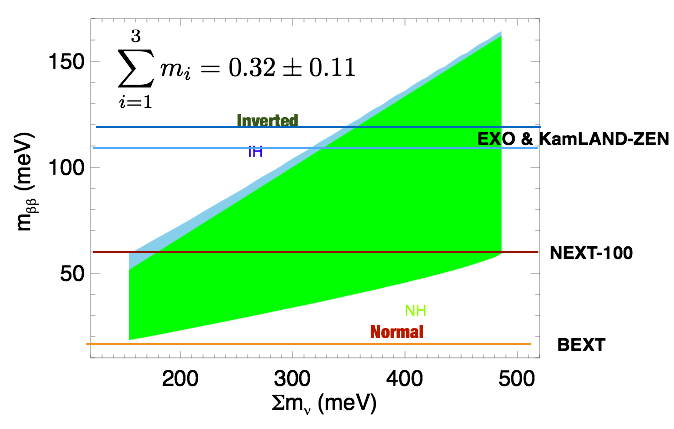
\includegraphics[width=0.75\textwidth]{img/SensiCRR.png}
\caption{\small The allowed \mbb\ region (68\% CL for two degrees of freedom), as a function of the sum of the neutrino masses, assuming that 
$\sum m_i = 0.32\pm 0.11$~eV. The blue lines mark the sensitivity of EXO and KamLAND-ZEN, the xenon-based detectors currently leading the field. The red line shows the sensitivity of NEXT after 3 years operation, which gives the experiment a sizable chance of making a discovery.} 
\label{fig.mbb}
\end{figure}
%%%%%%

 Several analyses from recent cosmological results suggest that the sum of the masses of the three neutrinos could be $\sim$ 0.3 eV\footcite{PhysRevLett.112.051303}. The PI and collaborators have demonstrated that, in this case, if the neutrino is a Majorana particle, then, $\mbb \sim [20-150]$~ meV \footcite{GomezCadenas:2013ue}, as shown in Figure \ref{fig.mbb}. In this scenario, the sensitivity of GERDA is outside the ``cosmologically relevant region'' (CRR), while both EXO-200 and KamLAND-Zen would have already explored a significant fraction of CRR {\em for the most optimistic NME set} (while they would be outside CRR for the most pessimistic). 
 
% Clearly, the experimental effort to determine if the neutrino is a Majorana particle, far from being completed is, rather, in its infancy. To establish unambiguously that the neutrino is (or not) a Majorana particle, even in this favourable scenario in which the sum of the neutrino masses is relatively high, experiments must be sensitive to $\mbb \sim 20$~meV, {\em even for the most pessimistic NME} set. On the other hand, a xenon experiment probing a $\Tonu >2.6 \times 10^{25}$~yr, has chances of making a discovery.
% 
 
%%%%%%%%%%%%%%%%%%%%%%%%%%%%%%%%%%%%%%%%%%%%%%%%%%%%%%%%%%%%
\paragraph{The NEXT experiment and its innovative concepts.}
\begin{figure}
\centering
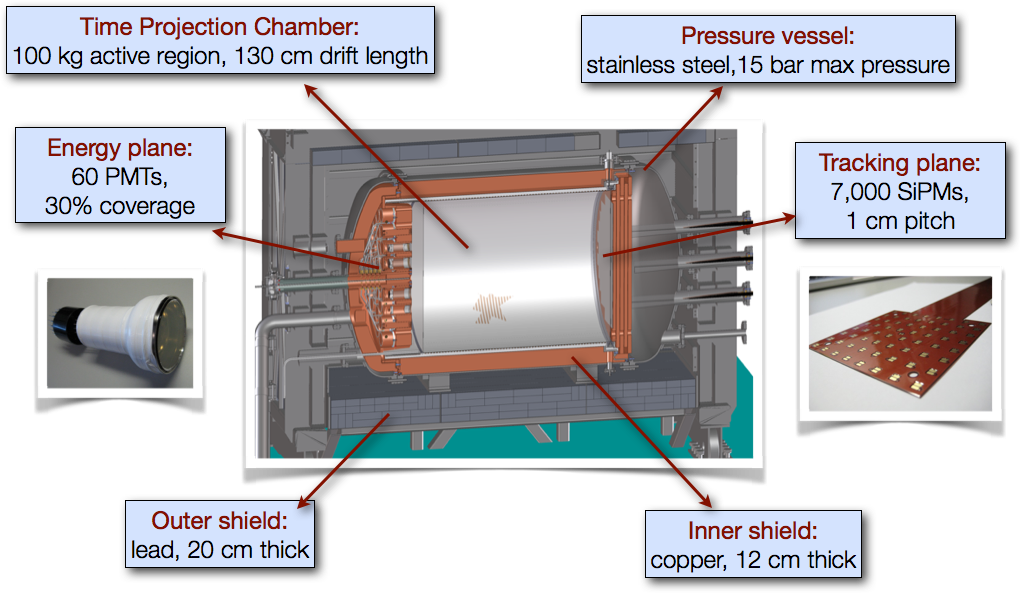
\includegraphics[width=0.9\textwidth]{img/NEXT.png}
\caption{\small A drawing of the NEXT-100 detector showing its main parts. The pressure vessel (PV) is made of a radio pure steel-titanium alloy. The PV dimensions are 130~cm inner diameter, 222~cm length, 1~cm thick walls, fot a total mass of 1\,200 kg. The inner copper shield (ICS) is made of ultra-pure copper bars and is 12~cm thick, with a total mass of 9\,000 kg. The time projection chamber includes the field cage, cathode, EL grids and HV penetrators.
The light tube is made of thin teflon sheets coated with TPB (a wavelength shifter). 
The energy plane is made of 60 PMTs housed in copper enclosures (cans).
The tracking plane is made of MPPCs arranged into dice boards (DB). 
} \label{fig.NEXT100}
\end{figure}

The \emph{Neutrino Experiment with a Xenon TPC} (NEXT)\footcite{next} will search for \bbonu\ in \XE\ using  high-pressure xenon gas  time projection chambers (\HPXE). The advantages of the technology are: 
a) {\bf excellent energy resolution}, with an intrinsic limit of about 0.3\% FWHM at \Qbb, close to that of \GE\ detectors; b)
{\bf tracking capabilities} that provide a powerful topological signature to discriminate between signal (two electron tracks with a common vertex) and background (mostly, single electrons); c)
{\bf a fully active and homogeneous detector}, with no dead regions; d) {\bf scalability} of the technique to large masses; e) the possibility of exciting the barium ion produced in the xenon decay from the fundamental state \TwoS\ to the state \TwoP, using a ``blue'' laser (493.54 nm), and observing the ``red light'' emitted in the transition from \TwoP\ to \TwoD, thus ``tagging'' the presence of a barium atom in the xenon gas, which cannot be produced by any known background. 

The design of the NEXT-100 detector (Figure \ref{fig.NEXT100}) is optimised for energy resolution by using proportional electroluminescent (EL) amplification of the ionisation signal. The detection process involves the use of the prompt scintillation light from the gas as start-of-event time, and the drift of the ionisation charge to the anode by means of an electric field ($\sim0.3$ kV/cm at 15 bar) where secondary EL scintillation is produced in the region defined by two highly transparent meshes, between which there is a field of $\sim20$ kV/cm at 15 bar. The detection of EL light provides an energy measurement using photomultipliers (PMTs) located behind the cathode (the \emph{energy plane}) as well as tracking through its detection a few mm away from production at the anode, via a dense array of silicon photomultipliers (the \emph{tracking plane}).

\paragraph{\label{sec.new}The NEW detector.}

%%%%%%%%%%
\begin{figure}
\centering
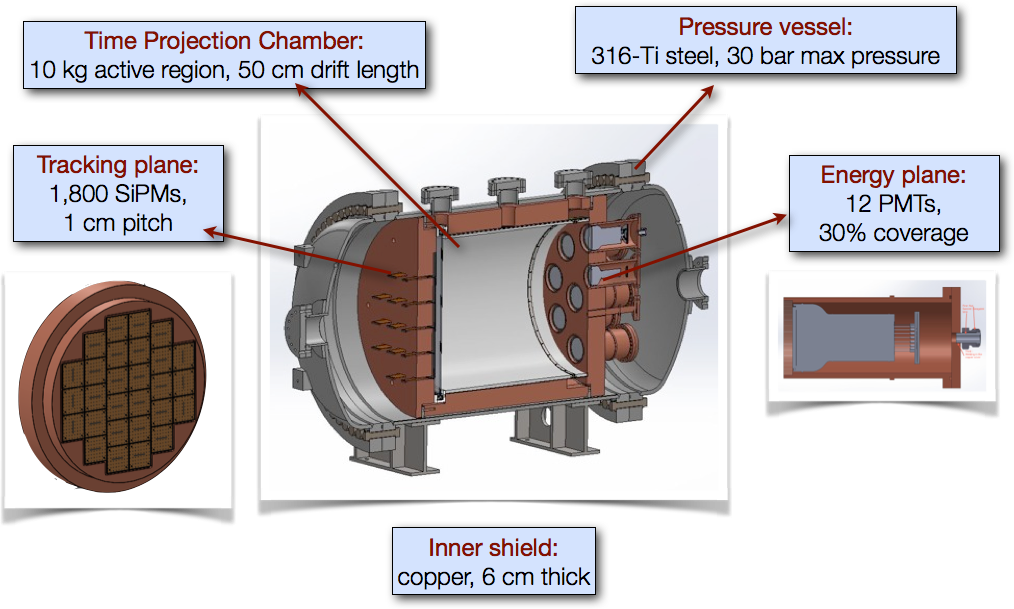
\includegraphics[height=9cm]{img/NEW.png}
\caption{\small The NEW apparatus.} \label{fig:NEW}
\end{figure} 

The NEW (NEXT-WHITE) apparatus\footnote{The name honours the memory of the late Professor James White, one of the key scientists of the NEXT Collaboration.}, shown in Figure \ref{fig:NEW}, is the first phase of the NEXT detector to operate underground. NEW 
%has a triple goal:
%
%\begin{enumerate}
%\item {\bf Technology}: it will validate the technological solutions adopted by NEXT-100.
%\item {\bf Radiopurity}: it will allow the NEXT collaboration an extra step in the implementation of a radiopure detector.
%\item {\bf Physics}: it will demonstrate with measurements of the \BI\ and \TL\ lines, as well as with the measurement of the \bbtnu\ spectrum, the physics capabilities of NEXT-100.
%\end{enumerate}
%
is a scale 1:2 in size (1:8 in mass) of NEXT-100. The energy plane contains 12 PMTs (20 \% of the 60 PMTs deployed in NEXT-100). The tracking plane technology consists of 30 Kapton Dice Boards (KDB) deploying 1800 SiPMs (also 20\% of the sensors). The field cage has a diameter of 50~cm and a length of 60~cm (the dimensions of the NEXT-100 field cage are roughly 1~m long and 1.2~m diameter). 

NEW is a necessary step\footnote{As formally stated by the scientific committee of the LSC, who recommended its construction in 2013.} towards the construction of NEXT-100. It will validate the technological solutions adopted by the collaboration and, as discussed below, it is essential in the definition of the project methodology. Furthermore, The NEXT background model is currently based on a sophisticated Monte Carlo simulation of all expected background sources in each part of the detector. NEW will allow the validation of the background model with actual data. 
%Last but not least, NEW operation will demonstrate with measurements of the \BI\ and \TL\ lines, as well as with the measurement of the \bbtnu\ spectrum, the physics capabilities of NEXT-100.

%Furthermore, the calibration of NEW with 
%sources of higher energy, will allow a precise study of the evolution of the resolution with the energy. 
%In particular it will be plausible to measure the resolution near \Qbb\ using a Thorium source, which provides 2.6 MeV gammas. Last, but not least, we intend to 
%reconstruct the spectrum of \bbtnu. Those events are topologically identical to signal events (\bbonu) and can be used to demonstrate with data the power of the topological signature. 
%
\paragraph{Discovery potential of NEXT-100.}

The excellent resolution of NEXT (0.5 \% FWHM), and the combination of a low radioactive budget with a topological signature (which yields an expected background rate of $5 \times 10^{-4} \ckky$), will allow the NEXT-100 detector to reach a sensitivity to the \bbonu\ period of $\Tonu > 7 \times 10^{25}$~yr for a exposure of 300 kg$\cdot$yr. This translates into a \mbb\ sensitivity range as low as $[67-187]$~meV, depending on the NME. Therefore NEXT-100 will have a substantial chance of making a discovery if the NME is sufficiently high (see Fig.~\ref{fig.mbb}). 

\paragraph{Towards a ton-scale high-pressure xenon TPC (BEXT).}

%%%%%%
\begin{figure}
\centering
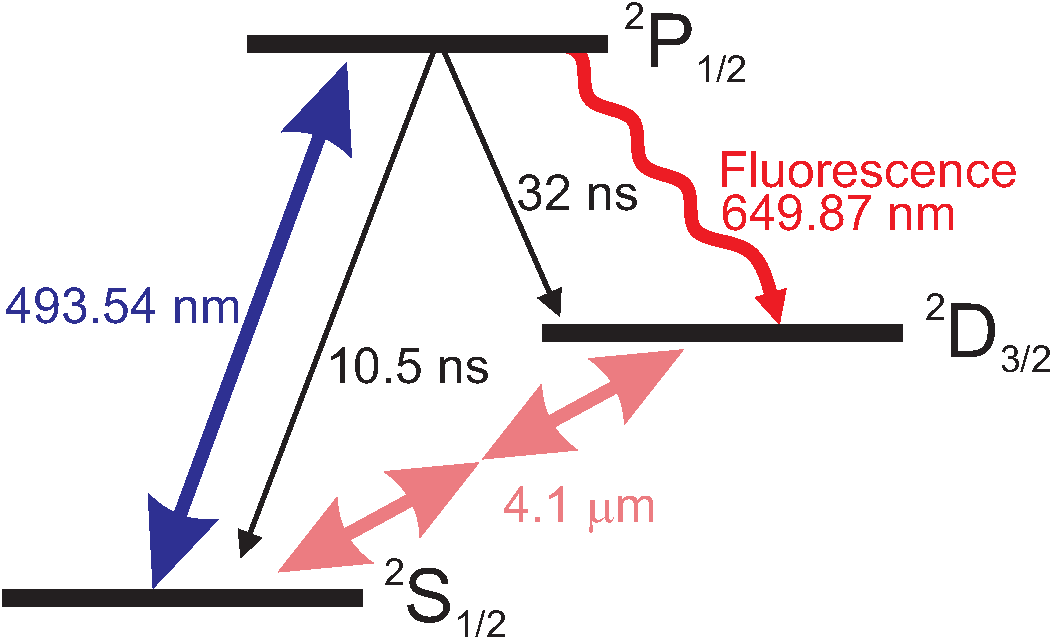
\includegraphics[width=0.50\textwidth]{img/levelscheme2.pdf}
\caption{\small The \BATA\ concept.} \label{fig.BATA}
\end{figure}
%%%%%%

If no discovery is made by the current generation of experiments, the full exploration of the CRR region (corresponding to the inverted hierarchy of neutrino masses, and \mbb\ values as low as 15~meV) requires detectors of larger mass (at least 1 ton), good resolution and extremely low specific background. The \HPXE\ technology has the potential to provide the most sensitive detector at this scale, by scaling the detector to a mass in the range of one ton and adding additional handles to further suppress the background. 

One of the most promising possibilities is to develop the technology to unambiguously tag the barium ion produced in the xenon decay, $Xe \rightarrow Ba^{++} + 2 e^-$. The conceptual idea to tag $Ba^{+}$ is illustrated in Figure \ref{fig.BATA}. A ``blue'' laser of wavelength 493.54 nm excites (``pumps'') the S state, inducing $S \rightarrow P$~transitions, with a lifetime of $\sim$ 10 ns. About 30 \% of the times the \TwoP\ states decay to the state \TwoD, emitting ``red'' (649.76 nm) fluorescence in a characteristic time of 30 ns. The state \TwoD\ is metastable, but a second laser of suitable wavelength (4.1 $\mu$m) can be used to induce the transition to the ground state (this is known as ``deshelving'').  The whole cycle takes less than 50 ns, and therefore several millions of red fluorescence photons can be emitted by a single ion. 

The practical application of this conceptual idea is by no means easy, and in fact, it has been shown to be extremely difficult in liquid xenon by the work of the EXO collaboration\footcite{Dolinski:2012dta}. However, it may be feasible in a \HPXE\ detector, where a number of fortunate conditions may occur. These conditions are: a) charge reduction of the emitted barium ion, from $Ba^{++}$~to $Ba^{+}$, which can be induced by collisions with xenon atoms, or by the addition of a suitable quencher; b) ``trapping'' of the barium ion ``in situ'' by the surrounding Xe atoms, which result in a very low drift velocity for the ion; c) location of the ion, via the reconstruction of the event topology. 

All the above needs to be demonstrated with a systematic R\&D program, which must also address additional experimental issues such as pressure broadening of the laser, filtering of Rayleigh scattering, and others. Most importantly, such an experimental program must be carried out by an interdisciplinary group, combining the experience in laser spectroscopy and atomic physics, with the experience in \HPXE\ instrumentation.

The on-going collaboration between the IFIC (and other groups of NEXT) and the Center for Pulsed Lasers (CLPU)\footcite{clpu}, a national facility dedicated to ultra-intense lasers, has made possible to create precisely the interdisciplinary team needed for a successful R\&D program, which can culminate in a ``Barium-tagging Experiment with a Xenon TPC'' (BEXT). 
A future detector of 1 ton mass, with a resolution of 0.5 \% FWHM and a background rate in the range of $10^{-6} \ckky$~(thanks to the implementation of barium-tagging) would be able to fully cover the CRR (and inverted hierarchy) region in less than 5 years, assuming a favourable scenario for the NME. Even the most pessimistic NME scenario could be fully explored, athough with a longer run, since the sensitivity to the \bbonu\ period increases linearly with exposure for a virtually background free experiment as in this case. 

Clearly the construction of a ton-scale \HPXE\ detector implementing the full \BATA\ technology is a very challenging enterprise. On the other hand, we believe that the incremental approach devised by the NEXT collaboration will work also in this case. The construction of the NEW detector is progressing without significant problems thanks to the expertise and know-how gained during the DEMO phase, and we expect that NEXT-100 will fully benefit from the experience gained with NEW. Similarly, the \BATA\ technology could be ready in a period of 4 years by approaching the problem step by step. This R\&D task can be carried out in parallel with the construction and commissioning of NEXT.
